\documentclass[12pt,a4paper]{article}
\usepackage[hmargin=0.8in,vmargin=0.8in]{geometry}\usepackage[T1]{fontenc}
\usepackage{graphicx}
\usepackage{url}
\usepackage{hyperref}
\hypersetup{hidelinks}

\usepackage{amsmath}
\usepackage[euler]{textgreek}

\setlength{\topskip}{0mm}\setlength{\parskip}{1em}\setlength{\parindent}{0em}
\usepackage{enumitem}\setlist{nolistsep}
\setlist[description]{style=nextline}
\usepackage{minted}

\usepackage{natbib}
\setlength{\bibsep}{0.0pt}

\usepackage{appendix}

\newcommand{\maxn}{max\textsuperscript{n}}
\newcommand{\Maxn}{Max\textsuperscript{n}}
\newcommand{\TDLeaf}{TDLeaf(\textlambda)}


\begin{document}
\begin{center}
    \textsc{The University of Melbourne\\
    School of Computing and Information Systems\\
    COMP30024 Artificial Intelligence}\\
    \vspace{1em}
    \textbf{\Large Project Part B: Report}\\
    \vspace{1em}
    Jin Han (843345), 
    \scalebox{0.1}{Mingda Dong (849313)}\footnotemark
\end{center}

\footnotetext{Drawn to scale.}

\section{Code structure}
% Briefly describe the structure of your game-playing program. 
% Give an overview of the major modules and/or
% classes you have created and used.

The game-playing programs consists of the following 3 components:

\subsection{Players}
  Players are the main component of the game-playing program,
all of which implicitly implement the ``\texttt{Player}'' interface with
the following 3 methods:
\begin{itemize}
    \item \mint{python}|def __init__(self, color: Color)|
    \item \mint{python}|def action(self) -> Action|
    \item \mint{python}|def update(self, color: Color, action: Action)|
\end{itemize}
Each of the player classes are responsible of maintaining the states and other
data that is needed by their respective algorithms, and use the algorithm to
make decisions.

\subsection{Board} \label{board}
\texttt{Board} class is an \textit{immutable and hashable} 
representation of the game state. A \texttt{Board} is defined by (a) all of 
the Chexer pieces on the board, distinguished only by their colors, and (b) 
the number of pieces that has exited the board per player.

Besides recording information, \texttt{Board} has also provided several useful
utility methods including (a) an iterator for possible actions by any player,
(b) generate another board using an Action tuple, (c) get the winner of current
board if available.

\subsection{Type definitions, constants, and other utilities} \label{typedef}
Utilising the fact
that Python 3.6 is used in this assignment, and considering the complexity of
this project, type annotations \cite{PEP484} are actively used in all 
methods. Several types that has special meanings, like \texttt{Coordinate},
\texttt{Action}, and \texttt{Color}, are given aliases for a clearer code
structure and preventing unintended type error while writing.

Also, other useful constants (number of pieces to exit to win, etc.) and 
utility functions (axial manhattan distance, etc.), which are being used
in multiple players, are also lifted out to common sub-namespaces.

\section{Strategy}
% Describe the approach your game-playing program uses for deciding on 
% which actions to take. Comment on your search strategy, including on how 
% you have handled the 3-player nature of the game. Explain your
% evaluation function and its features, including their strategic 
% motivations.
\subsection{Baseline Players}
Two baseline players are created to measure the performance of other players.
The \textit{Random Action Player} picks an action randomly from the list
of all possible actions in every round. The \textit{Simple Greedy Player}
picks the the action which brings any of its pieces closest to the exit hexes.

\subsection{\Maxn{} Player}
Another player is implemented using the \maxn{} algorithm \cite{Luckhardt1986}.

\Maxn{} is an adoption of minimax algorithm into multi-player games, where
instead of alternating minimum and maximum nodes in a search tree, the node
with maximum utility value of each player is chosen at their layers. 
In a \maxn{} search tree, each node has $n$ utility values for each player.

In our \maxn{} player, we have chosen the following features into 
consideration:

\begin{description}
    \item[\texttt{dist}] Number of steps for the 
        ``nearest candidates''\footnotemark{} to exit the board, assuming there 
        are no other pieces on the board. A shorter \texttt{dist} value 
        is better.
    \item[\texttt{n\_pieces\_exited}]  $\in [0, 4]$. Number of pieces the 
        player has exited from the board. States with more pieces 
        exited are preferred.
    \item[\texttt{n\_pieces\_to\_exit}] $\in [0, 4]$. Number of pieces needed 
        to exit to win the game. $4 - \texttt{n\_pieces\_exited}$
    \item[\texttt{n\_pieces\_missing}] $\in [0, 4]$. Number of pieces the player
        is lacking of to win the game. \\
        $\max(0, \texttt{n\textunderscore pieces\textunderscore to\textunderscore exit} - |\text{Pieces}|)$
    \item[\texttt{jump}] Number of \texttt{JUMP} actions possible in 
        this state. \texttt{JUMP} actions are particularly helpful in both
        moving faster to the exit hexes and converting pieces of enemies.  
    \item[\texttt{conv}] Number of pieces of other players can can convert
        our ``nearest candidates''. This attribute is used to minimise the
        chance where our pieces are converted by other opponents, especially
        when we are in short of pieces to win the game.
    \item[\texttt{coherence}] Number of ``nearest candidates'' that are next 
        to each other. Through observations, we found out that moving multiple
        pieces together and keep them next to each other is an efficient way
        to move forward with jumping and lower the chance of being converted
        by other players.
\end{description}

\footnotetext{``Nearest candidates'' are the $n$ pieces of the current player
that are nearest to his exit hexes. $n$ is determined by the number of pieces
needed to exit to win the game at the point of time.}

\section{Machine learning techniques}
% If you have applied machine learning, discuss the learning 
% methodology you followed for training and the
% intuition behind using that specific technique.
\subsection{Monte Carlo Tree Search} \label{mcts}
At the beginning, as an alternative strategy, we explored Monte Carlo Search 
Tree Search (MCTS) for Chexers Player. MCTS algorithm \cite{Nijssen2013}
is a search algorithm that randomly sample the search space through Monte
Carlo simulations, and going through the 
``selection-expansion-playout-backpropagation'' cycle to decide a move.
A significant advantage of MCTS is that it does not require an heuristic 
function to work, which has allowed us to quickly produce a usable agent
for benchmarking purpose.

\subsection{\TDLeaf} \label{tdleaf}

\TDLeaf{} algorithm is used to train the weights for our heuristic function
in the \maxn{} player. \TDLeaf{} \cite{Baxter1999} is an variant of 
TD(\textlambda) -- a reinforcement learning algorithm usually used with 
neural networks. \TDLeaf{}, however, are adapted to train weights of 
heuristic functions in a \textit{minimax} search algorithm. The agent is 
trained with hyperparameters $\lambda = 0.7, \eta = 1.0$.

\begin{align}
    r(s_i^l, w) & = \tanh(\text{eval}(s_i^l), w)\\
    d_i & = r(s_{i+1}^l, w) - r(s_i^l, w) \\ 
    w_j & \leftarrow w_j + \eta \sum_{i=1}^{N-1} 
    \left(
        \frac{\partial r(s_i^l, w)}{\partial w_j}
        \left(
            \sum_{m=1}^{N-1} \lambda^{m-i} d_m
        \right)
    \right)
\end{align}

Due to the nature of \TDLeaf{}, it is common to see that a weight set falls 
in a not-so-effective local optimum. We have also created a script to 
automate the process of training through self-playing, logging down the weight 
changes, detect convergence and re-seeding the initial weights. This has 
helped us to reach a better training result.

\section{Effectiveness}
% Comment on the overall effectiveness of your game-playing program. 
% If you have created multiple game-playing
% programs using different techniques, compare their relative effectiveness

\label{pruning}
On the \maxn{} player, we added both immediate pruning and shallow pruning
\cite{Sturtevant2000} for better performance. Both of the pruning techniques
are commonly used in \maxn{} searhes. Immediate pruning is to stop
searching whenever the heuristic value of a node is found with the maximum
value, in this case--when the player wins. Shallow pruning is to stop 
expanding a node when it knows that this node will not be chosen by examining
the current best heuristic value of its parent and the designed total maximum
value of all players.

\label{lazyeval}
Also, we implemented lazy evaluation so as to prevent unnecessary computation
when not needed. This is achieved by only compute the value when first 
accessed by \maxn{} algorithm through customized getters and setters in 
\texttt{Max\textsuperscript{n}\_Player.Score} class, which is also responsible
for the computation per se.

Through a one-vs-two tournament-like experiment among all agents we 
prepared, we have come out with the following ranking of effectiveness,
from the most effective one to the least:

\[
    \texttt{Tkinter}\footnote{Played by a human player.} > 
    \text{\Maxn{}}(3)\footnote{\Maxn{}($n$) indicates a search depth of $n$ layers.} > 
    \text{\Maxn{}}(2) > \text{Greedy} > \text{MCTS} > \text{Random}
\]

\section{Creative techniques}
% Include a discussion of any particularly creative techniques you have 
% applied (such as evaluation function design, search strategy optimisations, 
% specialised data structures, other optimisations, or any search algorithms
% not discussed in lectures) or any other creative aspects of your solution, 
% or any additional comments you wish to be considered by the markers.
\subsection{Algorithms}
In this project, we utilized various algorithms, training,
and optimisation techniques for a better performance, including MCTS 
(section \ref{mcts}), \TDLeaf{} (section \ref{tdleaf}), immediate and shallow
pruning (section \ref{pruning}).

\subsection{\texttt{Tkinter} Player}
In order to play the game and testing our agents within the team, we 
implemented an GUI player using Matt Farrugia's 
\texttt{texgen.py}\footnotemark{} based on \texttt{Tkinter} GUI library.

The \texttt{Tkinter} Player consist of 2 parts, a ``server'' that communicate
with the Referee, and a ``client'' that communicate with the user for game
status and moves. This design decision is made due to the fact that 
\texttt{Tkinter} window cannot run in a separate thread or non-blocking, which
is not feasible when working with the unmodified version of the Referee
program. ``Servers'' and ``clients'' communicate with the Python's built-in
XMLRPC protocol.

\begin{figure}[ht]
    \centering
    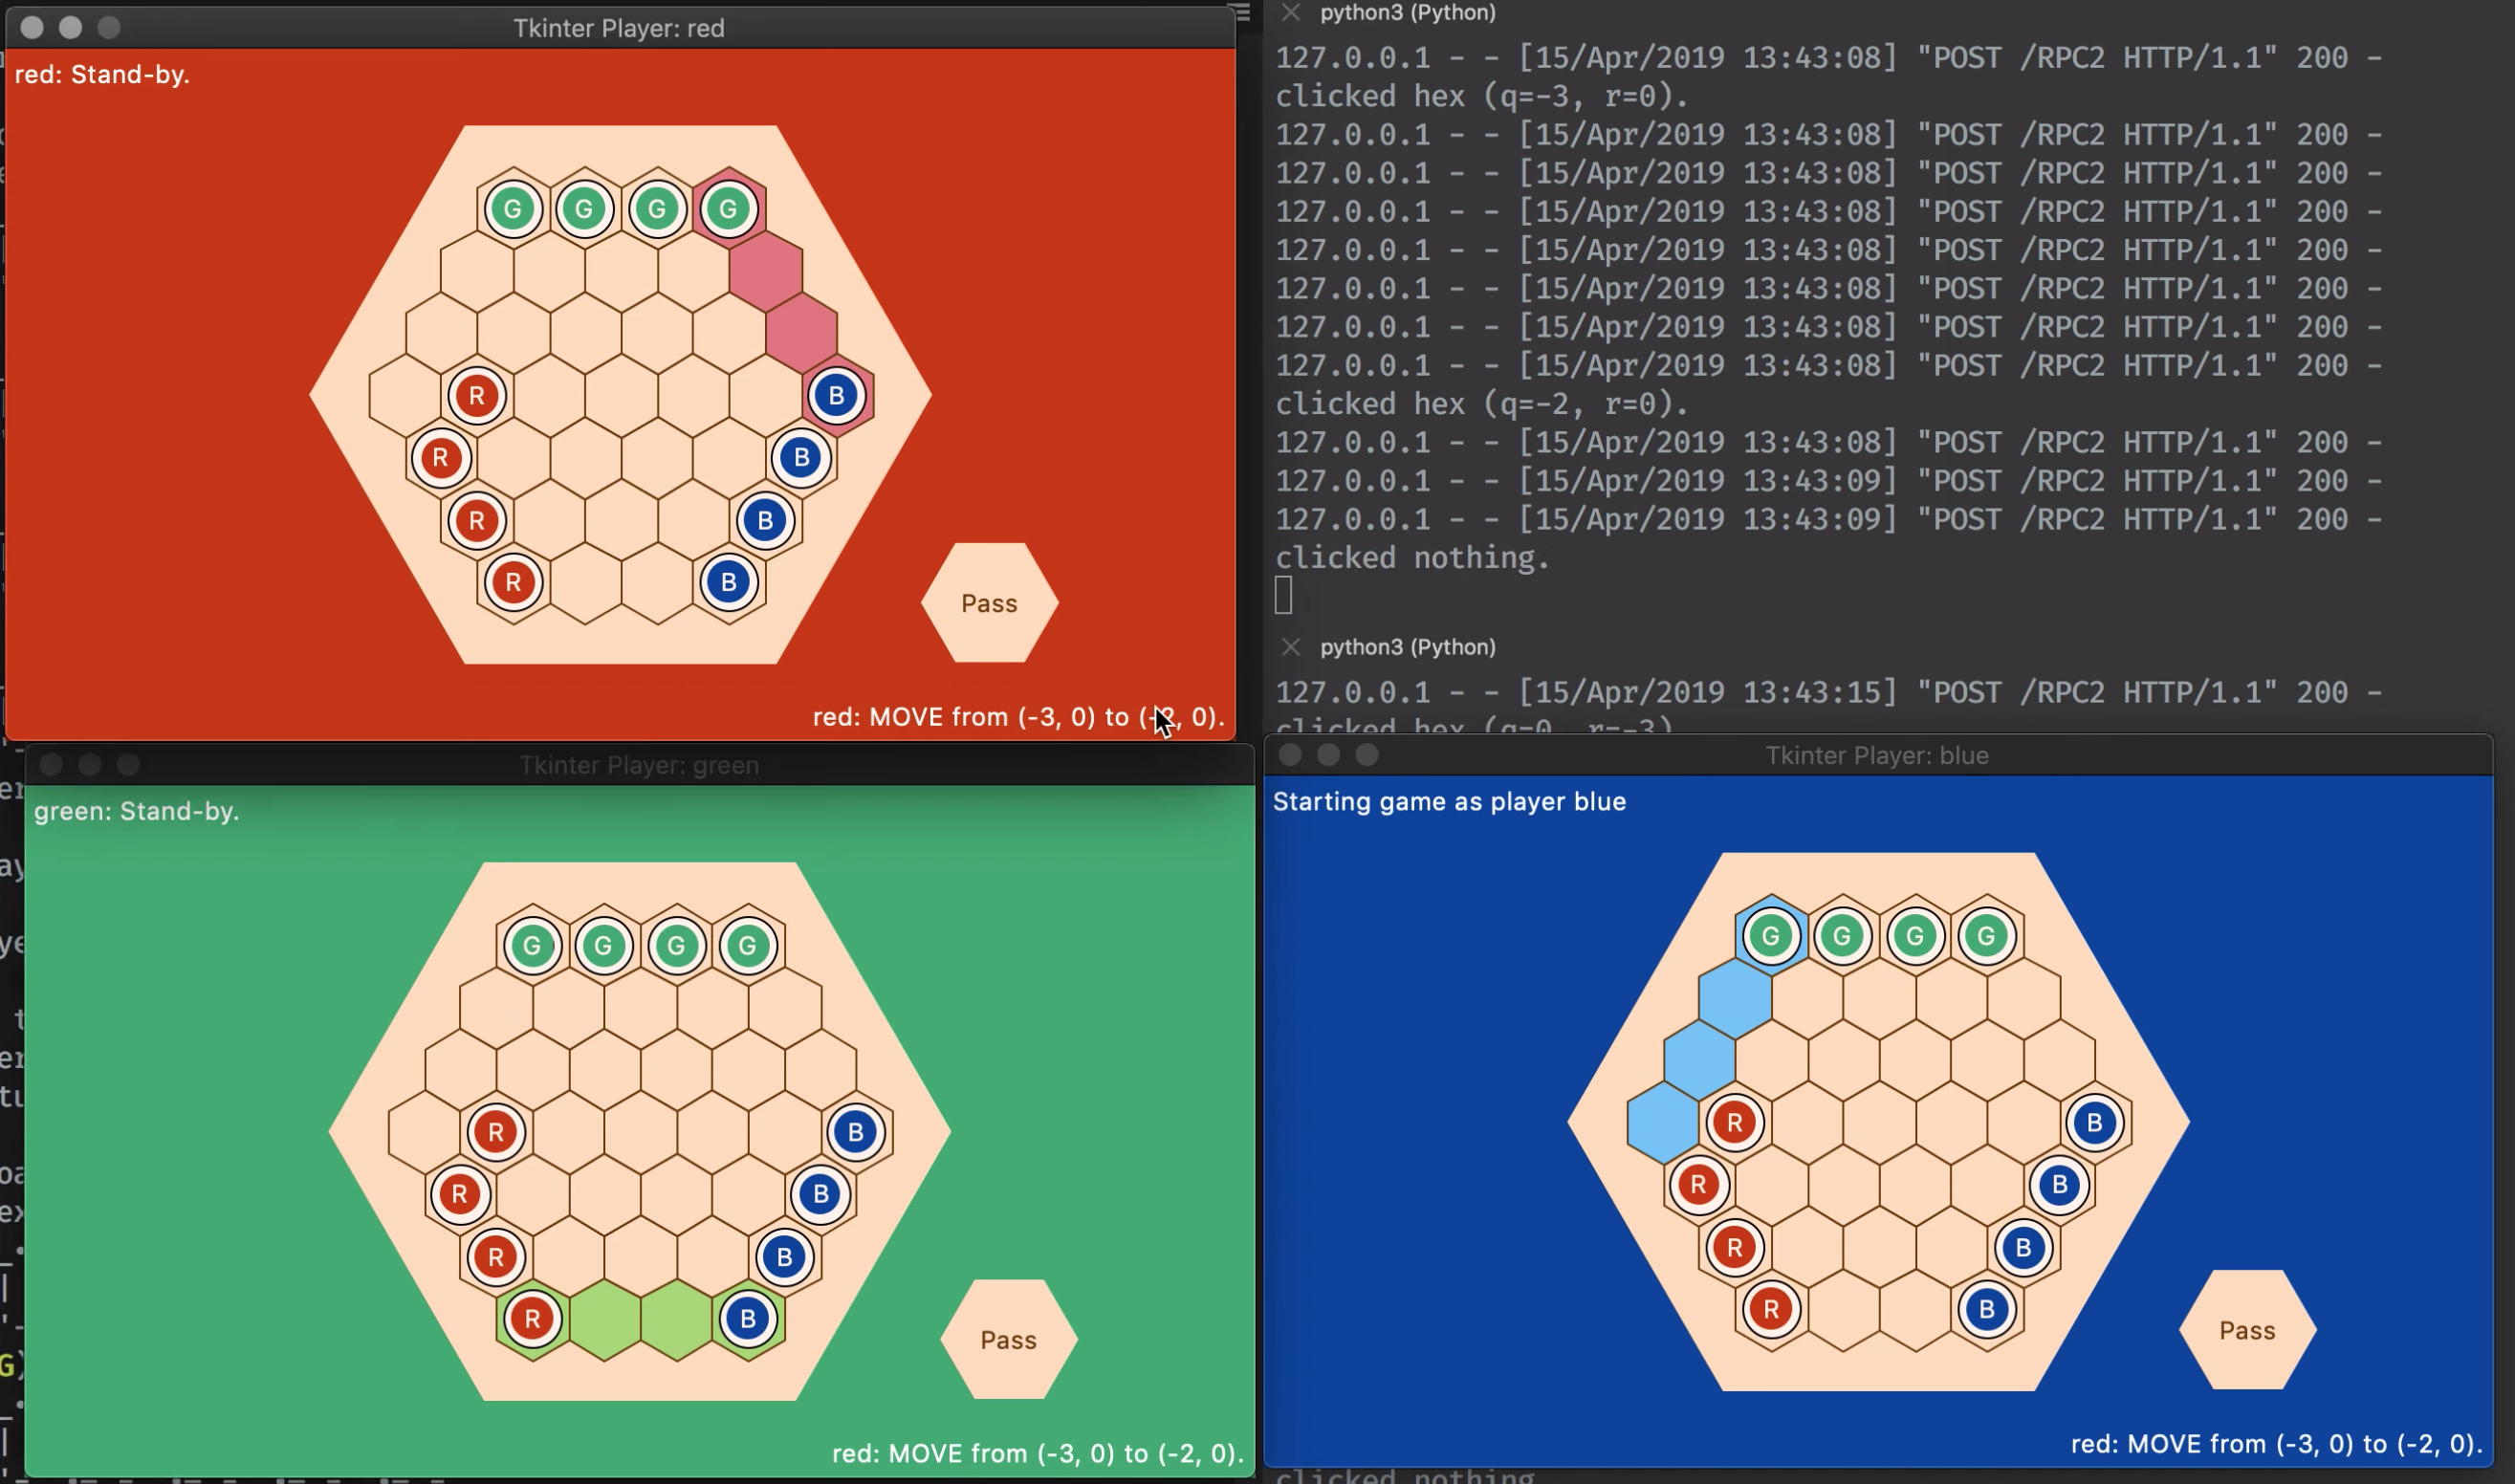
\includegraphics[height=7.5cm]{tkinter_player}
    \caption{Screenshot of \texttt{Tkinter} Players at work [\href{https://www.youtube.com/watch?v=0pAZfejTCMg}{YouTube}]}
\end{figure}


\footnotetext{\url{https://app.lms.unimelb.edu.au/webapps/discussionboard/do/message?action=list_messages&course_id=_382870_1&conf_id=_814031_1&forum_id=_455420_1&message_id=_1870319_1&nav=discussion_board_entry}}

\subsection{Miscellaneous}
In this project, we have implemented various data structures specially for
the game and some algorithms, including \texttt{Board} (section \ref{board}),
\texttt{Max\textsuperscript{n}\_Player.Score} (section \ref{lazyeval}), etc. 
Lazy evaluation (section \ref{lazyeval}) is also introduced for a more 
efficient computation. Also, other techniques such Type Hinting are also
utilized in the code (section \ref{typedef}). An automated script is also
written to speed up the training process for \TDLeaf{} (section \ref{tdleaf}).
Last but not least, we actively used Unicode mathematical notations in the 
source code, which makes it look more similar to what is shown in the report, 
reference papers, etc. 


\bibliographystyle{abbrv}
\bibliography{references}

\appendix
\appendixpage
\section{Git commit statistics}

\begin{table}[ht]
    \centering
    \begin{tabular}{l|rrr}
        & \textbf{Lines added} & \textbf{Lines deleted} & \textbf{Commits} \\ \hline
        Jin Han & $+4187$ & $-447$ & 30 \\ \hline
        Mingda Dong & $+44$ & $-13$ & 1
    \end{tabular}
    \caption{Git commit statistics}
\end{table}
\end{document}